\documentclass[11pt,a4paper]{article}

\usepackage[T1]{fontenc}
\usepackage[utf8]{inputenc}
\usepackage{lmodern}
\usepackage[margin=2.4cm]{geometry}
\usepackage{microtype}
\usepackage{booktabs}
\usepackage{multirow}
\usepackage{graphicx}
\usepackage{float}
\usepackage{subcaption}
\usepackage{amsmath}
\usepackage{amssymb}
\usepackage{siunitx}
\usepackage[dvipsnames]{xcolor}
\usepackage{tikz}
\usetikzlibrary{positioning,arrows.meta,decorations.pathreplacing,fit,backgrounds}
\usepackage[colorlinks=true,allcolors=NavyBlue!70!black]{hyperref}

\sisetup{detect-all, group-minimum-digits=4, group-digits=integer}

\newcommand{\rmse}{nRMSE}
\newcommand{\best}[1]{\textbf{#1}}
\newcommand{\reportone}{Report~I}

\title{\bfseries MRIxFields 2026: Progress Report II\\[0.3em]
\large Frequency-Band Methods, Volumetric Pretraining, and Synthetic Pair Generation}
\author{Berkin Deniz Kahya \and Furkan Yüceyalçın \and Racha Badreddine \and Ahmet Zelka}
\date{}

\begin{document}
\maketitle

\begin{abstract}
\noindent
Second progress report. It covers work completed since \reportone{}~\cite{report1} and reports only what
is new; results established there, in particular the control case and the spectral characterisation
of the dataset, are cross-referenced rather than repeated.

A second pass through the literature found the same mechanism in two otherwise unrelated systems.
UniField~\cite{lin2026unifield} and FPS-Former~\cite{meng2025fpsformer} both split the image spectrum
into low, mid and high bands and treat the bands differently, but they place the split in different
components: UniField puts it in the \emph{training loss}, as band-masked focal frequency terms with
hand-set weights, and FPS-Former puts it \emph{inside the attention block}, as a difference-of-Gaussians
pyramid whose per-band attention maps are summed before being applied to a shared value. This matters to
us because \reportone{} measured the quantity both of them approximate by hand. The per-transition change
in power-law exponent $\Delta\alpha$ is large only at \SI{0.1}{\tesla} ($+1.0$ to $+1.5$) and is near
zero or negative for every other source field, which says which band needs weight and where band
reweighting cannot help at all.

Three lines of work then respond to three properties of the challenge data. Because unpaired volumes are
abundant, we replaced the slice-wise LeJEPA encoder of \reportone{} with a volumetric Tubelet-ViT variant
on 16-slice slabs; pretraining runs and is stable, but the validation protocol is unrun and there is no
downstream transfer number yet. Because only three travelling-volunteer subjects supply real cross-field
pairs, we built a self-paired synthetic generator that degrades real \SI{7}{\tesla} volumes into
lower-field approximations through a SynthSeg-calibrated tissue-wise intensity remap, field-calibrated
blur, and Rician noise. Its first version reproduced field-specific appearance but collapsed
between-volume variability to \SIrange{11}{41}{\percent} of the real spread; after letting the target
tissue profile vary per sample, the ratios rise to \numrange{0.86}{0.98} at \SI{0.1}{\tesla},
\SI{3}{\tesla} and \SI{5}{\tesla}, with \SI{1.5}{\tesla} still lagging at \numrange{0.64}{0.66}. Because
band-separated architectures looked promising, we trained FPS-Former as a single shared Task~3 model.
At 30 epochs it improves on the StarGAN~v2 challenge baseline on \rmse{} (\num{0.284} versus
\num{0.344}) and SSIM (\num{0.865} versus \num{0.740}) but not on LPIPS (\num{0.156} versus
\num{0.155}), and it stays behind the conditional U-Net of \reportone{} (\num{0.236}, \num{0.901},
\num{0.089}) on all three.

We also scored a Task~3 control case, the unmodified input submitted as its own prediction. It reads
the same way \reportone{}'s Task~1 control did, and sharpens the FPS-Former result. The control loses
badly on \rmse{} (\num{0.522}) but scores SSIM \num{0.836}, \emph{beating} the challenge baseline by
\num{0.097}, and LPIPS \num{0.157}. FPS-Former therefore improves on doing nothing by \num{0.0011} of
LPIPS. Perceptual distance is where a frequency-aware model should have its advantage, and on that
metric it is indistinguishable from copying the input.
\end{abstract}

\section{Scope}
\label{sec:scope}

\reportone{} established three things this report builds on and does not re-derive.

\begin{itemize}
  \item \textbf{The control case.} A submission that returns the source volume unchanged scores
  \rmse{} \num{0.4085}, SSIM \num{0.8935}, LPIPS \num{0.0897}, Dice \num{0.8549} and volume consistency
  \num{0.8586} on Task~1, which is within noise of every trained challenge baseline on all metrics
  except \rmse{}. Any number reported below is therefore read against that control, not against the
  published baselines alone.
  \item \textbf{The spectral picture.} Radially averaged power spectra follow $P(f)\propto f^{-\alpha}$,
  and the exponent gap between a source field and \SI{7}{\tesla} is concentrated almost entirely at
  \SI{0.1}{\tesla}. Table~\ref{tab:dalpha} reproduces the per-transition figure, because
  Section~\ref{sec:thread} uses it directly.
  \item \textbf{The Task~3 reference points.} StarGAN~v2 as the challenge baseline, and a 10-epoch
  conditional U-Net that beats it on every metric.
\end{itemize}

\begin{table}[H]
  \centering
  \small
  \caption{$\Delta\alpha = \alpha_{\text{source}} - \alpha_{\SI{7}{\tesla}}$ on the retrospective split,
  from \reportone{}. Positive means the source spectrum falls off faster than the target's, so the model
  has to add high-frequency power. Only \SI{0.1}{\tesla} carries a substantial gap; three of the nine
  entries above it are negative, meaning the source already has \emph{more} high-frequency power than
  the target.}
  \label{tab:dalpha}
  \begin{tabular}{lccc}
    \toprule
    Source field & T1W & T2W & T2FLAIR \\
    \midrule
    \SI{0.1}{\tesla} & \best{$+1.009$} & \best{$+1.502$} & \best{$+1.294$} \\
    \SI{1.5}{\tesla} & $+0.158$ & $+0.100$ & $+0.350$ \\
    \SI{3}{\tesla}   & $-0.171$ & $-0.060$ & $+0.344$ \\
    \SI{5}{\tesla}   & $-0.505$ & $-0.214$ & $+0.182$ \\
    \bottomrule
  \end{tabular}
\end{table}

\section{Frequency-band separation in related work}
\label{sec:lit}

\subsection{UniField: the band split in the loss}
\label{sec:unifield2}

UniField is covered in detail in \reportone{}, and only the part that Section~\ref{sec:thread} needs is
recalled here. It trains a single latent flow-matching model for all modalities and both of its field
transitions, and adds to the velocity-matching objective a band-masked focal frequency term,
\begin{equation}
  \mathcal{L}_{\text{FASFL}} = \lVert v_\theta - v \rVert_1
  + \lambda_{\text{freq}} \sum_{b \in \{\text{low},\text{mid},\text{high}\}}
  \frac{w_b}{|M_b|} \big\lVert M_b \odot |\Delta F|^{\alpha} \odot |\Delta F|^{2} \big\rVert_1,
  \qquad \Delta F = F(v_\theta) - F(v),
  \label{eq:fasfl}
\end{equation}
with $M_b$ a binary mask selecting band $b$. The band weights are set by hand from a physical argument:
$w_b = [0.2, 0.5, 0.3]$ for \SI{64}{\milli\tesla}$\rightarrow$\SI{3}{\tesla}, where the high band is
down-weighted because the target's fine detail has no counterpart in the source and penalising it invites
hallucination, and $w_b = [0.1, 0.3, 0.6]$ for \SI{3}{\tesla}$\rightarrow$\SI{7}{\tesla}, where the low
band is down-weighted to stop the model reproducing B1 inhomogeneity. The network itself is generic; the
band structure lives entirely in the loss.

\subsection{FPS-Former: the band split in the attention block}
\label{sec:fpsformer}

FPS-Former~\cite{meng2025fpsformer} targets accelerated MRI reconstruction from undersampled k-space:
hierarchical encoder--decoder ViT, plain $L_1$ loss, data-consistency layer. Since multi-head
self-attention is low-pass, it splits the features into frequency bands \emph{inside} the attention
block (Figure~\ref{fig:fmam}):
\begin{equation}
  \begin{aligned}
    \text{FMAM:}\quad X_m &= G_{\sigma_m} \ast F_{\text{in}},
      & \qquad T_m &= X_{m+1} - X_m, \\
    S_m &= \sum_{i=1}^{I} \operatorname{softmax}\!\big(Q^i_m K_m^{i\top}/\sqrt{d}\big),
      & \qquad F_f &= \Big(\sum_{m=1}^{M} S_m\Big) V
  \end{aligned}
\end{equation}
\begin{equation}
  \text{SPAM:}\quad Z_j = \big\lfloor (a^\top f_j + b)/r \big\rfloor, \qquad
    F_p = \operatorname{unsort}\big(\operatorname{MSA}(\mathcal{G}_n)\big), \qquad
    F_{\text{out}} = f\big([F_p,\, F_f]\big),
\end{equation}
with $\sigma_1 < \dots < \sigma_{M+1}$, so $T_m$ is a difference-of-Gaussians band-pass; $Q_m, K_m$
from $T_m$ and $V$ from the unsplit $F_{\text{in}}$; $a \sim \mathcal{N}(0,1)^C$,
$b \sim \mathcal{U}(0,r)$, so $\mathcal{G}$ are locality-sensitive hash buckets and $f$ is a depthwise
convolution. The two remaining modules are a $3\times3 / 5\times5$ depthwise feed-forward network and a
mixture of CNN experts.

\begin{figure}[H]
  \centering
  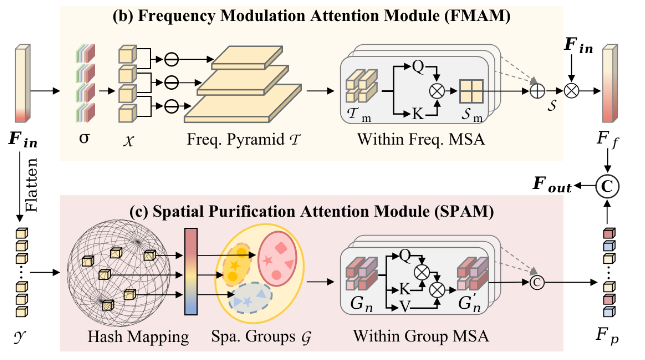
\includegraphics[width=0.82\linewidth]{figures/fpsformer_attention.png}
  \caption{FPS-Former's two attention modules, reproduced from~\cite{meng2025fpsformer}. FMAM (top)
  builds a difference-of-Gaussians pyramid from the features and runs multi-head self-attention within
  each band, summing the maps before applying them to a value taken from the unsplit input. SPAM
  (bottom) hashes tokens into spatial groups and attends within a group. Only FMAM is relevant to our
  setting.}
  \label{fig:fmam}
\end{figure}

\paragraph{Transferability.} Only FMAM, with two caveats. Its premise is that the missing high
frequencies are measured but undersampled, so they exist in k-space and the data-consistency layer can
enforce them; translation has neither, and at \SI{0.1}{\tesla} the content is absent rather than
aliased (\reportone{}). And the bands are defined on feature maps per stage, not on the image spectrum,
so the correspondence to a measured $\Delta\alpha$ is qualitative.

\subsection{Common feature: separation of frequency bands}
\label{sec:thread}

Figure~\ref{fig:bands} places the two mechanisms side by side. Both treat a single undifferentiated
objective over the whole spectrum as the wrong granularity, on the grounds that the low, mid and high
bands need different treatment. They differ in where the split is applied: UniField
reweights the \emph{error} per band and leaves the architecture generic; FPS-Former reweights the
\emph{representation} per band and leaves the loss generic. The two are not mutually exclusive, and
nothing prevents combining them.

UniField's $w_b$ are six hand-set numbers standing in for a measurable property of the data, and
Table~\ref{tab:dalpha} is that measurement. It also bounds where band reweighting can act: only the
\SI{0.1}{\tesla} transition has a substantial positive $\Delta\alpha$, and three of the nine
higher-field entries are \emph{negative}, meaning the source already carries more high-frequency power
than the \SI{7}{\tesla} target and a high-band bonus would push the model the wrong way. A band-weighted
loss with a fixed $w_b$ shared across all transitions would therefore be actively harmful above
\SI{1.5}{\tesla}; if we adopt one, the weights have to be conditioned on the transition and derived from
the measured $\Delta\alpha$, with the sign respected.

\begin{figure}[H]
  \centering
  \resizebox{\linewidth}{!}{%
  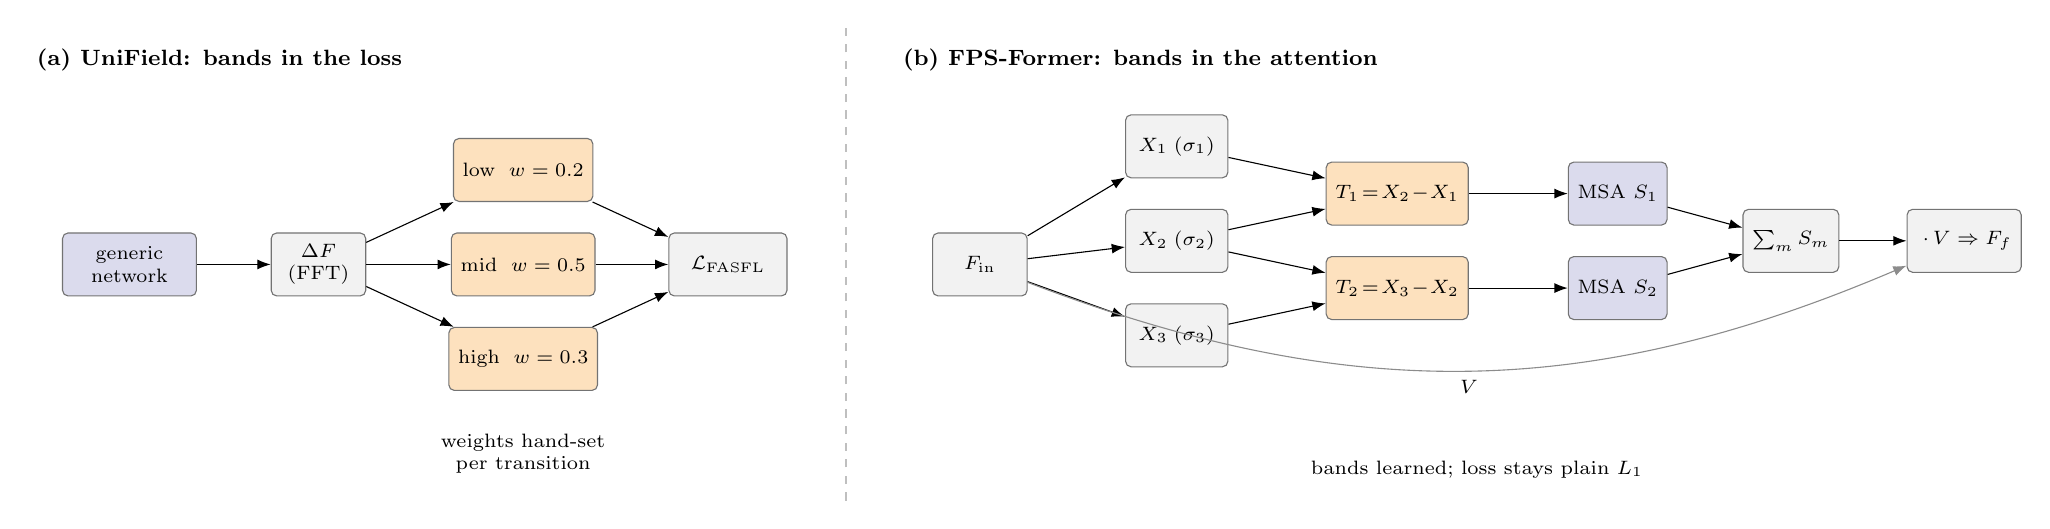
\begin{tikzpicture}[
    >=Latex,
    font=\small,
    blk/.style={draw=black!55, rounded corners=2pt, minimum height=8mm, align=center, font=\scriptsize},
    gen/.style={blk, fill=black!5},
    act/.style={blk, fill=BurntOrange!22},
    net/.style={blk, fill=NavyBlue!14},
  ]
    \node[font=\bfseries\footnotesize, anchor=west] at (-0.4, 2.6) {(a) UniField: bands in the loss};

    \node[net, minimum width=17mm] (net1) at (0.9,0) {generic\\network};
    \node[gen, minimum width=12mm] (dF)  at (3.3,0) {$\Delta F$\\(FFT)};
    \node[act, minimum width=13mm] (bl)  at (5.9,1.2) {low $\;w=0.2$};
    \node[act, minimum width=13mm] (bm)  at (5.9,0)   {mid $\;w=0.5$};
    \node[act, minimum width=13mm] (bh)  at (5.9,-1.2){high $\;w=0.3$};
    \node[gen, minimum width=15mm] (L)   at (8.5,0)   {$\mathcal{L}_{\text{FASFL}}$};

    \draw[->] (net1) -- (dF);
    \foreach \b in {bl,bm,bh} { \draw[->] (dF) -- (\b); \draw[->] (\b) -- (L); }
    \node[font=\scriptsize, align=center, text width=32mm] at (5.9,-2.4)
      {weights hand-set per transition};

    \draw[black!25, dashed] (10.0,-3.0) -- (10.0,3.0);

    \node[font=\bfseries\footnotesize, anchor=west] at (10.6, 2.6)
      {(b) FPS-Former: bands in the attention};

    \node[gen, minimum width=12mm] (fin) at (11.7,0) {$F_{\text{in}}$};
    \node[gen, minimum width=13mm] (x1) at (14.2,1.5) {$X_1\;(\sigma_1)$};
    \node[gen, minimum width=13mm] (x2) at (14.2,0.3) {$X_2\;(\sigma_2)$};
    \node[gen, minimum width=13mm] (x3) at (14.2,-0.9){$X_3\;(\sigma_3)$};
    \node[act, minimum width=15mm] (t1) at (17.0,0.9) {$T_1\!=\!X_2\!-\!X_1$};
    \node[act, minimum width=15mm] (t2) at (17.0,-0.3){$T_2\!=\!X_3\!-\!X_2$};
    \node[net, minimum width=11mm] (s1) at (19.8,0.9) {MSA $S_1$};
    \node[net, minimum width=11mm] (s2) at (19.8,-0.3){MSA $S_2$};
    \node[gen, minimum width=11mm] (sum) at (22.0,0.3) {$\sum_m S_m$};
    \node[gen, minimum width=12mm] (ff) at (24.2,0.3) {$\;\cdot\,V \Rightarrow F_f$};

    \foreach \x in {x1,x2,x3} \draw[->] (fin) -- (\x);
    \draw[->] (x1) -- (t1); \draw[->] (x2) -- (t1);
    \draw[->] (x2) -- (t2); \draw[->] (x3) -- (t2);
    \draw[->] (t1) -- (s1); \draw[->] (t2) -- (s2);
    \draw[->] (s1) -- (sum); \draw[->] (s2) -- (sum);
    \draw[->] (sum) -- (ff);
    \draw[->, black!45] (fin) to[bend right=22] node[midway, below, font=\scriptsize, black] {$V$} (ff);
    \node[font=\scriptsize, align=center, text width=42mm] at (18.0,-2.6)
      {bands learned; loss stays plain $L_1$};
  \end{tikzpicture}}
  \caption{Two placements of the same idea. (a) UniField masks the spectral residual into three bands and
  weights the resulting error terms with hand-set, transition-specific $w_b$; the network is unchanged.
  (b) FPS-Former builds a difference-of-Gaussians pyramid inside the attention block, computes an
  attention map within each band, and sums them before applying the result to a value taken from the
  unsplit features; the loss is unchanged. Redrawn from the descriptions
  in~\cite{lin2026unifield,meng2025fpsformer}.}
  \label{fig:bands}
\end{figure}

\section{Constraints and solution proposals}
\label{sec:three}

The remaining sections are organised by the property of the data that motivated each piece of work
rather than by author. Three properties are relevant, each implying a different approach.

\begin{enumerate}
  \item Unpaired volumes are plentiful and cover all fifteen field$\times$modality domains, so a
  representation can be learned without any pairing at all (Section~\ref{sec:encoder}).
  \item Real cross-field pairs are almost absent, so pairs can be manufactured from the volumes we do
  have (Section~\ref{sec:synth}).
  \item The published systems of Section~\ref{sec:lit} suggest concrete architectures, so one of them can
  be run on our data (Section~\ref{sec:fps}).
\end{enumerate}

\subsection{Volumetric encoder for unpaired data}
\label{sec:encoder}

\reportone{} pretrained a slice-wise LeJEPA encoder and found no clear ordering between LeJEPA, DINO and
random initialisation on Task~1. Two limitations of that setup were structural rather than tuning issues:
a slice-wise encoder cannot use through-plane continuity, and its patch features were trained only
indirectly through a pooled CLS objective, while the downstream translator consumes dense tokens. The
volumetric variant changes the input representation and the tokenizer and keeps the objective.

\paragraph{Views.} A base sample is a contiguous axial slab
$s_n = [x_z, \dots, x_{z+15}] \in [0,1]^{1\times16\times H\times W}$. Two global views are
$1\times16\times224\times224$ and six local views are contiguous 8-slice sub-slabs at
$1\times8\times96\times96$ with distinct depth offsets, each containing the common anchor anatomy.
Every view keeps the same subject, field strength and modality; one crop and affine transform is sampled
per view and applied coherently to all of its slices. Augmentations are restricted to small rotations,
translations, mild blur and mild Gaussian noise. Colour jitter, grayscale conversion, solarisation and
aggressive contrast changes are excluded on purpose, because field strength and modality appearance are
exactly the signal the downstream translator needs.

\paragraph{Tokenizer and encoder.} The stem is a non-overlapping 3D convolution,
\begin{equation}
  \mathcal{P}(X) = \operatorname{Conv3D}_{k = s = (2,16,16)}(X),
  \qquad C_{\text{out}} = 768,
\end{equation}
so a global view becomes an $8\times14\times14$ token grid (1568 tokens) and a local view a
$4\times6\times6$ grid (144 tokens). A learned CLS token is prepended and a standard ViT-B (12 blocks, width 768, 12 heads, MLP ratio
4) processes every view with shared weights. Positional encoding is a learned absolute 3D table,
trilinearly interpolated for the local and downstream grids, with the CLS position kept separate.
Interpreting the tubelet's depth axis as ordered anatomy rather than time is the only substantive
departure from the video precedents~\cite{avjepa,vjepa,videomae}; it is not a masked-latent-prediction
method, so it is LeJEPA with a 3D stem and not V-JEPA.

\paragraph{Objective.} There are $V_g = 2$ global and $V = 8$ total views. Write
$z_{n,v} = g_\phi\big(f_\theta(v_{n,v})_{\text{CLS}}\big) \in \mathbb{R}^{128}$ for the projected
embedding of view $v$ of sample $n$, with $g_\phi$ a shared BatchNorm MLP of widths
$768 \to 2048 \to 2048 \to 128$, and $\mu_n = V_g^{-1}\sum_{v \le V_g} z_{n,v}$ for the per-sample
global centre. Only the projected CLS enters the loss, which is~\cite{lejepa}
\begin{equation}
  \mathcal{L}_{\text{LeJEPA}}
  = (1-\lambda)\underbrace{\frac{1}{BV}\sum_{n,v}\lVert z_{n,v}-\mu_n\rVert_2^2}_{\mathcal{L}_{\text{inv}}}
  + \lambda\underbrace{\frac{1}{V|\mathcal{A}|}\sum_{v}\sum_{a\in\mathcal{A}}
    T_{\text{EP}}\big(\{a^\top z_{n,v}\}_{n=1}^{B}\big)}_{\mathcal{L}_{\text{SIGReg}}},
  \qquad \lambda = 0.05,
\end{equation}
with $T_{\text{EP}}$ the Epps--Pulley Gaussianity statistic over 1024 random directions and a 17-point
quadrature, and no stop-gradient on the centre or either encoder path. SIGReg is computed across the
physical batch of each view separately; correlated views are not flattened into the sample axis.

\paragraph{Data and export.} Self-supervision uses the retrospective cohort only, so the prospective
paired subjects stay unseen by both pretraining and any later supervised fine-tuning. Sampling is
hierarchical, uniform over the fifteen domains, then over volumes, then over valid 16-slice intervals,
which prevents the domains with more eligible windows from dominating. Intensities stay in $[0,1]$
through view construction and are mapped to the encoder range by $x_{\text{enc}} = 2x - 1$; no per-volume
standardisation, histogram matching or field-specific normalisation is applied, since those would erase
the acquisition appearance the translator needs. Only the tubelet encoder is exported. The projector and
SIGReg are training-only, and a downstream consumer receives post-LayerNorm dense features
$F \in \mathbb{R}^{B\times8\times h\times w\times768}$, adds source-field, target-field and modality
conditioning outside the SSL encoder, and fine-tunes the whole backbone.

\paragraph{Status.} Pretraining runs and optimisation is stable: losses stay finite and no collapse has
been observed in the loss curves. That is the extent of what can currently be claimed. The three-part
validation the design calls for is unrun, namely (i) collapse diagnostics beyond the loss, including
feature standard deviation, singular spectra and effective rank
$\operatorname{Rank}_{\text{eff}}(Z) = \exp(-\sum_k p_k \log p_k)$ with
$p_k = \sigma_k / \sum_j \sigma_j$; (ii) related-view retrieval and coordinate-matched dense-token
correspondence, which is the part that actually tests whether dense features retain anatomy; and (iii)
the causal transfer test comparing an identical downstream model initialised from this encoder against
random initialisation. A stable loss curve is consistent with a collapsed or anatomically uninformative
representation, so no transfer claim is made here. Given the \reportone{} result, where the ordering
between initialisations flipped depending on which metric was consulted, (iii) is the only one of the
three that settles anything, and it is the one that has not been run.

\begin{figure}[H]
  \centering
  \resizebox{0.96\linewidth}{!}{%
  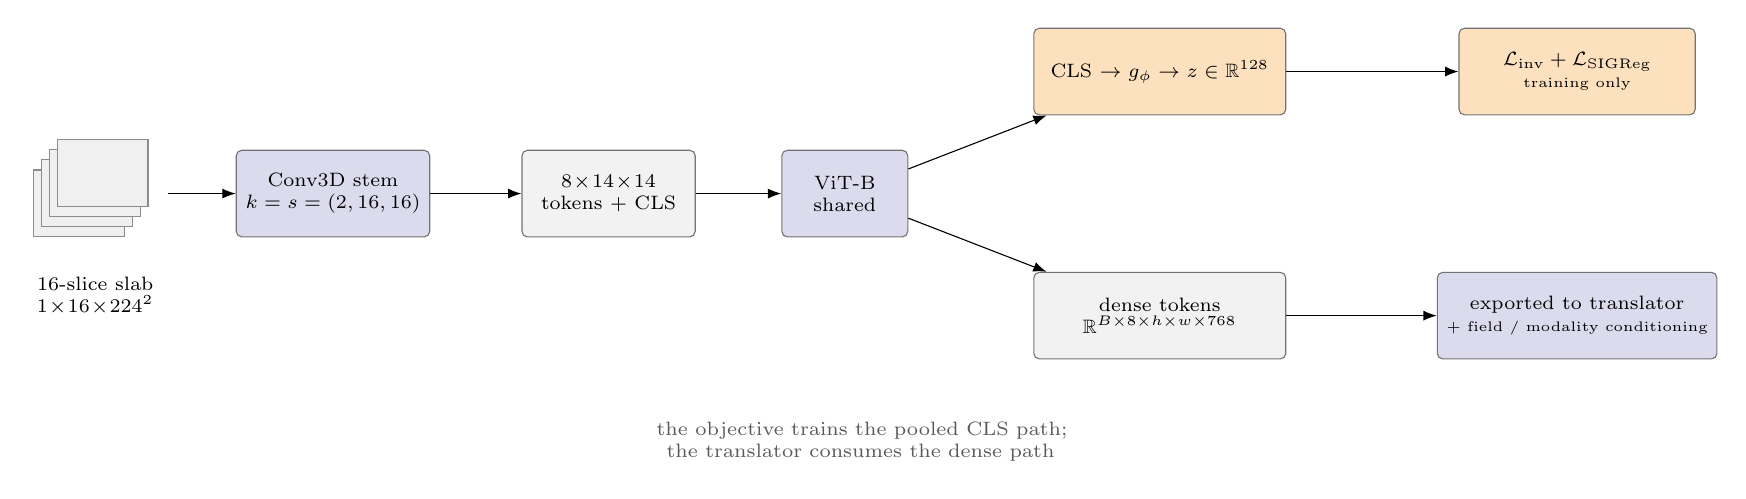
\begin{tikzpicture}[
    >=Latex,
    font=\small,
    blk/.style={draw=black!55, rounded corners=2pt, minimum height=11mm, align=center,
                font=\scriptsize},
    gen/.style={blk, fill=black!5},
    net/.style={blk, fill=NavyBlue!14},
    act/.style={blk, fill=BurntOrange!22},
  ]
    \foreach \i in {0,1,2,3}
      \draw[draw=black!45, fill=black!6] (0.10*\i, 0.13*\i) rectangle ++(1.15,0.85);
    \node[font=\scriptsize, align=center] at (0.78,-0.75) {16-slice slab\\$1\!\times\!16\!\times\!224^2$};

    \node[net, minimum width=24mm] (stem) at (3.8,0.55) {Conv3D stem\\$k=s=(2,16,16)$};
    \node[gen, minimum width=22mm] (grid) at (7.3,0.55) {$8\!\times\!14\!\times\!14$\\tokens $+$ CLS};
    \node[net, minimum width=16mm] (vit)  at (10.3,0.55) {ViT-B\\shared};

    \node[act, minimum width=32mm] (cls)  at (14.3,2.1)
      {CLS $\to g_\phi \to z\in\mathbb{R}^{128}$};
    \node[gen, minimum width=32mm] (dense) at (14.3,-1.0)
      {dense tokens\\$\mathbb{R}^{B\times8\times h\times w\times768}$};

    \node[act, minimum width=30mm] (loss) at (19.6,2.1)
      {$\mathcal{L}_{\text{inv}} + \mathcal{L}_{\text{SIGReg}}$\\{\tiny training only}};
    \node[net, minimum width=30mm] (down) at (19.6,-1.0)
      {exported to translator\\{\tiny $+$ field / modality conditioning}};

    \draw[->] (1.7,0.55) -- (stem);
    \draw[->] (stem) -- (grid);
    \draw[->] (grid) -- (vit);
    \draw[->] (vit) -- (cls);
    \draw[->] (vit) -- (dense);
    \draw[->] (cls) -- (loss);
    \draw[->] (dense) -- (down);
    \node[font=\scriptsize, align=center, text width=100mm, black!65] at (10.5,-2.6)
      {the objective trains the pooled CLS path; the translator consumes the dense path};
  \end{tikzpicture}}
  \caption{Tubelet-ViT LeJEPA. A 16-slice slab is tokenized by a $2\times16\times16$ Conv3D stem into an
  $8\times14\times14$ grid and encoded by a shared ViT-B. Only the projected CLS enters the
  self-supervised objective; the dense post-LayerNorm tokens are what the downstream translator receives.
  The gap between those two paths is the design's main open risk and the reason the dense diagnostics
  matter.}
  \label{fig:tubelet}
\end{figure}

\subsection{Synthetic paired data generation}
\label{sec:synth}

\subsubsection{Motivation}

Supervised translators need an input and a matching target. In this challenge only three
travelling-volunteer subjects provide scans across all required field strengths, which is not enough to
train one from real pairs. The move is to construct pairs in the direction we can control: start from a
real retrospective \SI{7}{\tesla} volume, degrade it into a synthetic lower-field approximation, and pair
that synthetic source with the \emph{original} \SI{7}{\tesla} volume it came from. The pairing is exact
by construction, since both sides are the same anatomy on the same voxel grid. This is the Image Quality
Transfer setup~\cite{alexander2017iqt}, with the low-quality side generated rather than acquired, and it
is intended as pretraining, to be followed by fine-tuning on the small set of real paired
travelling-volunteer data.

The risk is the synthetic-to-real domain gap. If the synthetic lower-field images do not statistically
resemble real lower-field scans, the model learns a mapping that does not apply to the challenge data.
And because this is medical image synthesis, plausible intensities are not sufficient: anatomy has to
survive the degradation. The generator therefore has to be validated on tissue intensity, noise,
resolution, diversity and anatomical consistency \emph{before} it is used, which is what the rest of this
section reports.

\subsubsection{Calibration}

The reference set is 15 real retrospective \SI{7}{\tesla} volumes; the target statistics come from 25
real retrospective volumes at each of \SI{0.1}{\tesla}, \SI{1.5}{\tesla}, \SI{3}{\tesla} and
\SI{5}{\tesla}. SynthSeg~\cite{billot2023synthseg} supplies soft tissue maps $p_t$ for
$t \in \{\text{CSF}, \text{GM}, \text{WM}\}$, and all statistics are tissue-weighted rather than global,
\begin{equation}
  \mu^{B}_{t} = \frac{\sum_v p_t(v)\,x(v)}{\sum_v p_t(v)},
  \qquad
  \big(\sigma^{B}_{t}\big)^2
    = \frac{\sum_v p_t(v)\,\big(x(v) - \mu^{B}_{t}\big)^2}{\sum_v p_t(v)},
\end{equation}
for each field $B$, and identically for the \SI{7}{\tesla} reference. Using tissue-conditional statistics
rather than a single global mean or histogram is the physically motivated choice here: $T_1$, $T_2$ and
$T_2^\ast$ all vary with $B_0$ \emph{and} differ between tissues, so CSF, GM and WM do not move together
as $B_0$ changes, and a single global transform cannot represent that.

\subsubsection{Degradation operator}

Four steps are applied in order to a real \SI{7}{\tesla} volume $x$.

\paragraph{1. Tissue-aware intensity remap.} Each tissue is remapped by a $z$-score transfer from the
\SI{7}{\tesla} statistics to the target-field statistics, blended toward the identity by a strength $s$
and composited with the soft tissue weights:
\begin{equation}
  x_1(v) = \sum_{t} p_t(v)\Big[(1-s)\,x(v) + s\Big(\mu^{B}_{t} + \sigma^{B}_{t}\,
  \frac{x(v) - \mu^{\SI{7}{\tesla}}_{t}}{\sigma^{\SI{7}{\tesla}}_{t} + \varepsilon}\Big)\Big]
  \;+\; \Big(1 - \min\big(1, \textstyle\sum_t p_t(v)\big)\Big)\,x(v).
  \label{eq:remap}
\end{equation}
The trailing term returns background and non-brain voxels unchanged, where the tissue posteriors sum to
approximately zero. Note that Equation~\ref{eq:remap} is a convex combination only where
$\sum_t p_t(v) \le 1$: the tissue sum in the first term is not renormalised while the residual term uses
the clipped sum, so any voxel at which the three posteriors over-sum receives total weight greater than
one. With three disjoint tissue classes this is rare, but it is a plausible contributor to the residual
intensity bias reported below and is worth removing.

\paragraph{2. Field-dependent blur.} $x_2 = G_\sigma \ast x_1$ with
$\sigma \sim \mathcal{U}[\sigma^{B}_{\min}, \sigma^{B}_{\max}]$, the range calibrated by comparing the
radially averaged power spectra of real source-field volumes against the \SI{7}{\tesla} reference over
the fit band of \reportone{}. This stands in for the loss of effective spatial detail at lower field,
where tissue boundaries and fine structures are less sharply resolved.

\paragraph{3. Rician noise.} MRI magnitude images are Rician, not Gaussian, so noise is added in the
complex plane before the magnitude is taken:
\begin{equation}
  x_3 = \sqrt{(x_2 + n_1)^2 + n_2^2},
  \qquad n_1, n_2 \stackrel{\text{iid}}{\sim} \mathcal{N}(0, \sigma_n^2),
\end{equation}
which is the standard magnitude-image model~\cite{gudbjartsson1995rician}. The per-field range for
$\sigma_n$ is estimated from real scans with a robust high-pass estimator: with residual
$r = x - G_1 \ast x$ and foreground $\Omega$,
\begin{equation}
  \hat{\sigma}_n = 1.4826 \cdot \operatorname{median}_{v \in \Omega}
  \big| r(v) - \operatorname{median}(r) \big|,
\end{equation}
optionally excluding the highest-gradient voxels so anatomical edges are not counted as noise. Two
caveats on this estimator, both of which bias it downward and both of which bite hardest at
\SI{0.1}{\tesla}. The high-pass residual retains only a fraction
$\lVert \delta - g_1 \rVert_2 \approx 0.95$ of white-noise energy for an isotropic 3D Gaussian with
$\sigma = 1$, so $\hat{\sigma}_n$ underestimates $\sigma_n$ by roughly \SI{5}{\percent}; and the
$1.4826$ MAD-to-$\sigma$ conversion assumes Gaussianity, which the Rician magnitude only approaches at
high SNR. Both push the calibrated noise slightly low precisely where the real scans are noisiest.

\paragraph{4. Clip.} $x_4 = \operatorname{clip}(x_3, 0, 1)$, matching the normalisation of the rest of
the dataset.

\paragraph{Stochasticity.} The remap strength $s$, the blur $\sigma$ and the noise $\sigma_n$ are sampled
independently per call from the calibrated field-specific ranges, so repeated degradation of the same
\SI{7}{\tesla} volume yields different but individually plausible lower-field versions. This is
deliberate and physically motivated: a \SI{7}{\tesla} volume does not correspond to one unique low-field
image, since loss of detail, noise and acquisition variability all make many lower-field appearances
compatible with the same underlying anatomy.

\begin{figure}[H]
  \centering
  \resizebox{0.98\linewidth}{!}{%
  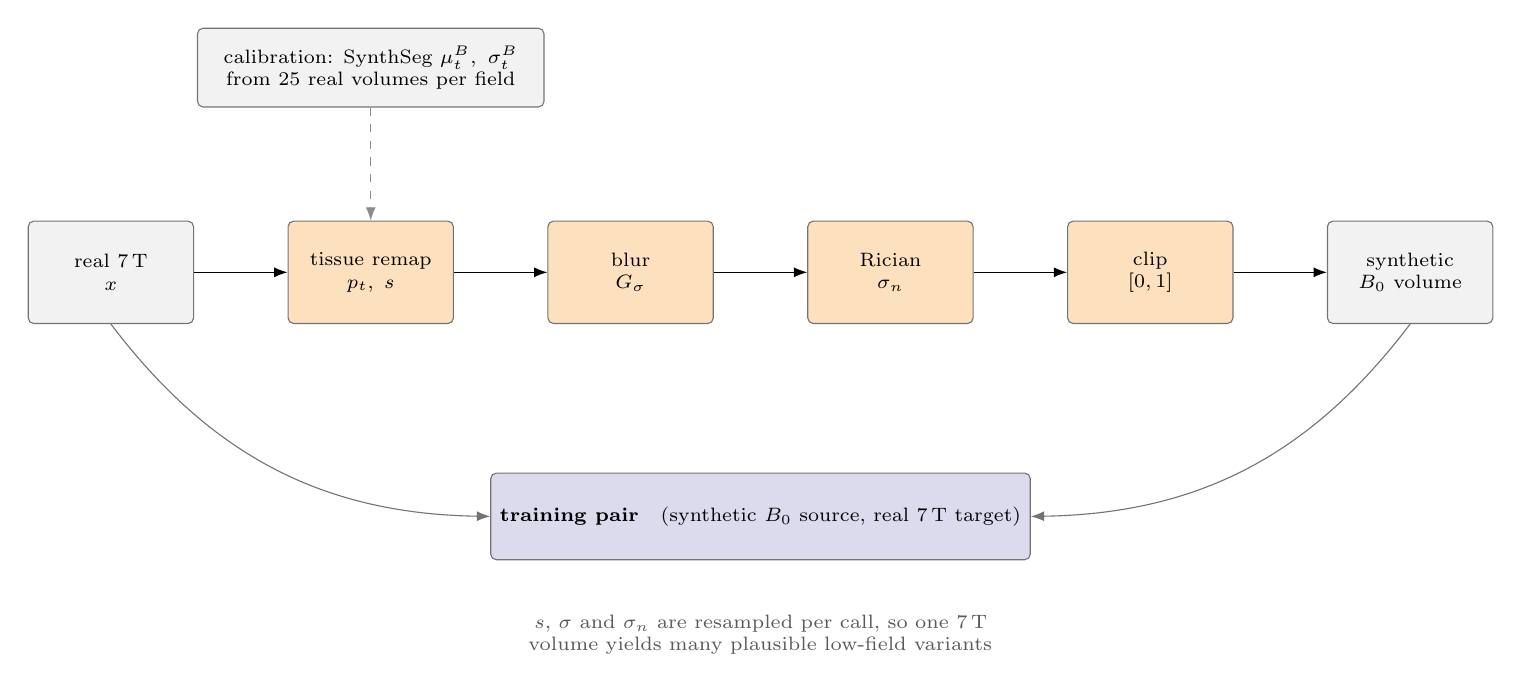
\begin{tikzpicture}[
    >=Latex,
    font=\small,
    blk/.style={draw=black!55, rounded corners=2pt, minimum height=13mm, minimum width=21mm,
                align=center, font=\scriptsize},
    gen/.style={blk, fill=black!5},
    act/.style={blk, fill=BurntOrange!22},
    net/.style={blk, fill=NavyBlue!14},
  ]
    \node[gen] (x)  at (0,0)    {real \SI{7}{\tesla}\\$x$};
    \node[act] (r)  at (3.3,0)  {tissue remap\\$p_t,\;s$};
    \node[act] (b)  at (6.6,0)  {blur\\$G_\sigma$};
    \node[act] (n)  at (9.9,0)  {Rician\\$\sigma_n$};
    \node[act] (c)  at (13.2,0) {clip\\$[0,1]$};
    \node[gen] (y)  at (16.5,0) {synthetic\\$B_0$ volume};

    \foreach \a/\b in {x/r, r/b, b/n, n/c, c/y} \draw[->] (\a) -- (\b);

    \node[net, minimum width=62mm, minimum height=11mm] (pair) at (8.25,-3.1)
      {\textbf{training pair}\quad (synthetic $B_0$ source, real \SI{7}{\tesla} target)};
    \draw[->, black!55] (x.south) to[bend right=26] (pair.west);
    \draw[->, black!55] (y.south) to[bend left=26]  (pair.east);

    \node[font=\scriptsize, align=center, text width=80mm, black!65] at (8.25,-4.6)
      {$s$, $\sigma$ and $\sigma_n$ are resampled per call, so one \SI{7}{\tesla} volume yields many
       plausible low-field variants};

    \node[gen, minimum width=44mm, minimum height=10mm] (cal) at (3.3,2.6)
      {calibration: SynthSeg $\mu^B_t,\ \sigma^B_t$\\from 25 real volumes per field};
    \draw[->, black!45, dashed] (cal) -- (r);
  \end{tikzpicture}}
  \caption{Synthetic pair generation. A real \SI{7}{\tesla} volume is degraded by a calibrated
  tissue-aware remap, blur and Rician noise, and the result is paired with the volume it was generated
  from. The pairing is exact by construction; what has to be validated is whether the left-hand side
  resembles a real low-field scan.}
  \label{fig:synthpipe}
\end{figure}

\subsubsection{Initial generator: validation results}

Validation compared 25 real retrospective volumes per source field against 45 synthetic volumes per
field, generated as three variants from each of the 15 \SI{7}{\tesla} references.

Two problems appeared. The smaller one is a systematic intensity bias: in all twelve
field$\times$tissue combinations the synthetic tissue mean fell below the real tissue mean, worst in the
lower fields, with \SI{0.1}{\tesla} gray matter low by \num{0.0478} and \SI{0.1}{\tesla} white matter low
by \num{0.0387}.

The larger one is that the synthetic volumes were far too similar to one another. Measuring the
between-volume spread of tissue means,
\begin{equation}
  m_{n,t} = \frac{\sum_v p_t(v)\,x_n(v)}{\sum_v p_t(v)},
  \qquad
  r_{B,t} = \frac{\operatorname{sd}_n\big(m^{\text{syn}}_{n,t}\big)}
                 {\operatorname{sd}_n\big(m^{\text{real}}_{n,t}\big)},
\end{equation}
gave $r_{B,t}$ between \num{0.108} and \num{0.409}: the synthetic scans varied only
\SIrange{11}{41}{\percent} as much as the real ones. The cause is structural rather than a tuning error.
A single average profile per field was estimated once, and every synthetic volume was then pushed toward
that same target appearance, so the generator had one attractor per field and the sampled $s$, $\sigma$
and $\sigma_n$ could only perturb around it.

For pretraining this is the more damaging of the two failures. A model pretrained on a low-variance input
distribution sees a narrow slice of appearance space and has no reason to become robust to the real
spread, which is exactly the property the pretrain-then-finetune plan depends on.

\subsubsection{Corrected generator}

The correction keeps the comparison pool and the random seeds fixed and changes one thing: the target
tissue profile is allowed to vary across synthetic samples instead of being pinned to a single per-field
average, so different generated volumes aim at different plausible points of the field's appearance
distribution rather than all at its mean.

Table~\ref{tab:diversity} gives the effect. At \SI{0.1}{\tesla} the three tissue ratios rise from the
range $0.23$--$0.29$ to $0.92$--$0.98$, and \SI{3}{\tesla} and \SI{5}{\tesla} move to \num{0.855} or
above. \SI{1.5}{\tesla} improves by a similar factor but from a lower base and ends at $0.64$--$0.66$,
still visibly short of the real spread; it is the one field that needs further field-specific tuning.

\begin{table}[H]
  \centering
  \small
  \caption{Synthetic-to-real between-volume standard deviation ratios $r_{B,t}$, before and after the
  correction. A value near \num{1} means the synthetic set reproduces the case-to-case variability of the
  real set. Same comparison pool and same seeds in both columns.}
  \label{tab:diversity}
  \begin{tabular}{llcc}
    \toprule
    Field & Tissue & Initial generator & Corrected generator \\
    \midrule
    \multirow{3}{*}{\SI{0.1}{\tesla}} & CSF & 0.294 & 0.983 \\
     & GM & 0.273 & 0.940 \\
     & WM & 0.232 & 0.916 \\
    \midrule
    \multirow{3}{*}{\SI{1.5}{\tesla}} & CSF & 0.223 & 0.664 \\
     & GM & 0.197 & 0.638 \\
     & WM & 0.157 & 0.661 \\
    \midrule
    \multirow{3}{*}{\SI{3}{\tesla}} & CSF & 0.409 & 0.855 \\
     & GM & 0.286 & 0.884 \\
     & WM & 0.283 & 0.898 \\
    \midrule
    \multirow{3}{*}{\SI{5}{\tesla}} & CSF & 0.273 & 0.942 \\
     & GM & 0.138 & 0.916 \\
     & WM & 0.108 & 0.940 \\
    \bottomrule
  \end{tabular}
\end{table}

\begin{figure}[H]
  \centering
  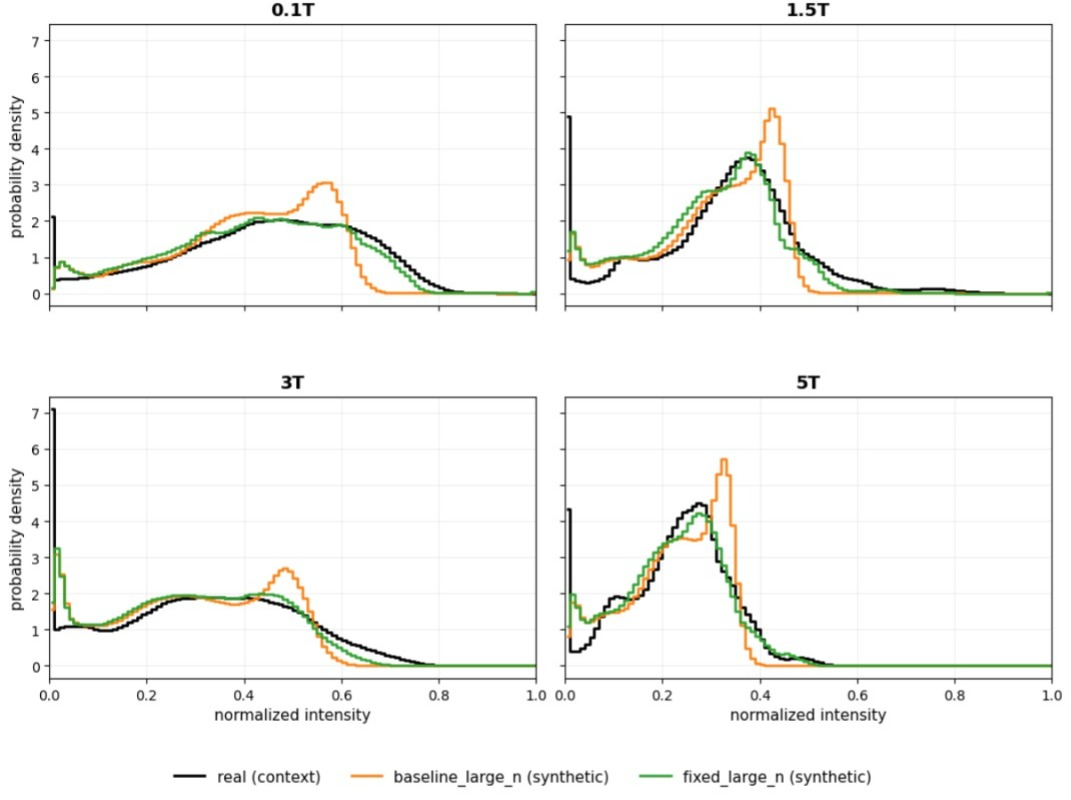
\includegraphics[width=0.86\linewidth]{figures/synth_tissue_histograms.png}
  \caption{Foreground intensity distributions for real (black), initial synthetic (orange) and corrected
  synthetic (green) volumes, per source field. The initial generator's narrow, displaced mode is visible
  at every field; the corrected generator tracks the real distribution's location and width much more
  closely, most clearly at \SI{0.1}{\tesla} and \SI{5}{\tesla}. This is a full-volume histogram and is
  dominated by the background peak near zero, so it supports but does not establish the conclusion; the
  tissue-level statistics of Table~\ref{tab:diversity} are the stronger evidence, and neither measures
  anatomical fidelity or spatial resolution.}
  \label{fig:synthhist}
\end{figure}

\begin{figure}[H]
  \centering
  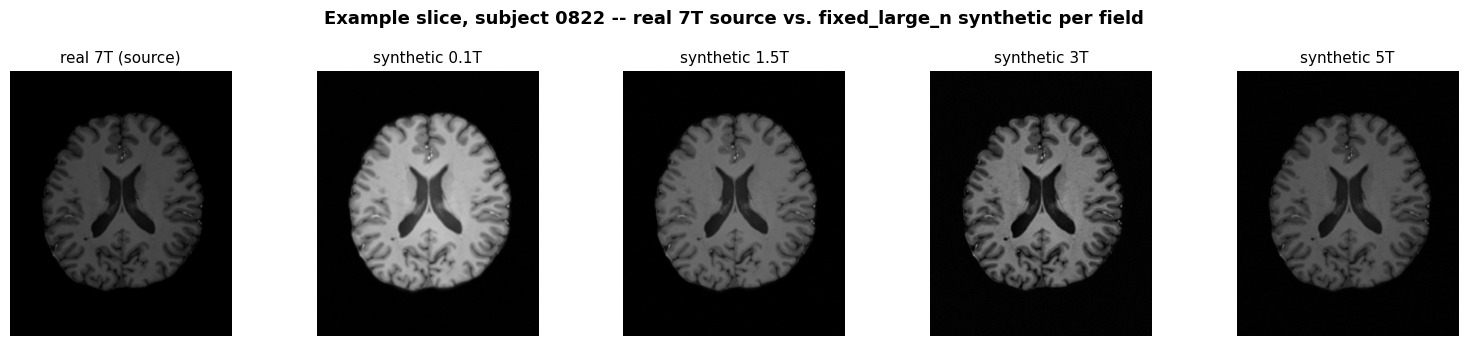
\includegraphics[width=\linewidth]{figures/synth_example_slices.png}
  \caption{One axial slice of subject 0822: the real \SI{7}{\tesla} source and the four synthetic
  lower-field volumes generated from it by the corrected generator. Anatomy is preserved by construction,
  since every voxel keeps its position; what varies is contrast, sharpness and noise. The
  \SI{0.1}{\tesla} panel is visibly the most degraded, consistent with it being the only transition with
  a substantial $\Delta\alpha$ in Table~\ref{tab:dalpha}.}
  \label{fig:synthslices}
\end{figure}

\paragraph{Remaining issues.} The intensity bias survives the correction: synthetic tissue means remain
slightly below real ones in most cases. That was left as the lower priority because a systematic offset
is a milder problem for pretraining than a collapsed variance, and because the non-convex compositing
noted under Equation~\ref{eq:remap} and the downward-biased $\hat{\sigma}_n$ are both candidate causes
worth eliminating before tuning anything. Two things have not been measured at all. Neither the histogram
nor the tissue statistics say anything about \emph{anatomical} consistency, which is what a
segmentation-based check on the synthetic volumes would test; and the spectral criterion the blur was
calibrated against has not been re-verified on the corrected output, so we do not yet know that the
corrected generator still matches real low-field power spectra. Finally, no model has been pretrained on
this data yet, so the premise of the whole exercise, that synthetic pretraining transfers, remains
untested.

\subsection{FPS-Former on Task 3}
\label{sec:fps}

One shared FPS-Former was trained across all modalities and all field translations as a single Task~3
model, in the same any-to-any setting as the conditional U-Net of \reportone{}. The configuration
follows the published one wherever the paper specifies a value: $M = 3$ frequency-pyramid levels in
FMAM, an SDFN expansion ratio of $2.0$, $E = 8$ experts per HEFR module, attention heads
$(1, 2, 4, 8)$ across the four stages, and four early and four final HEFR modules. FPS stage depths
are $(1, 2, 2, 1)$, giving 11 FPS blocks in total, at a base width of 48.

Pyramid depth is worth singling out, since it is the parameter the mechanism turns on: $M = 3$ is both
the paper's own setting and the optimum of its ablation, where smaller and larger $M$ each degraded
reconstruction, too few levels failing to separate the bands and too many confusing the aggregation.
Neither it nor any other listed value is a divergence, so the configuration does not account for the
result below.

The one deviation is ours: a token cap in the attention modules, 256 for FMAM and 128 for SPAM, added
to bound memory. It also bounds how much context either module attends over, and its effect on the
result has not been measured. Table~\ref{tab:task3} gives the 30-epoch validation result against the
two existing reference points.

\begin{table}[H]
  \centering
  \small
  \caption{Task~3, averaged over modalities. StarGAN~v2 and the conditional U-Net are from \reportone{}
  and the experiment log; the control case and FPS-Former are new. The control case is the unmodified
  input volume submitted as its own prediction, scored on the platform like any other entry. The
  trained runs are not matched on budget or schedule, so that comparison is not controlled.}
  \label{tab:task3}
  \begin{tabular}{lcccl}
    \toprule
    Model & \rmse{}~$\downarrow$ & SSIM~$\uparrow$ & LPIPS~$\downarrow$ & Note \\
    \midrule
    Control case & 0.5216 & 0.8365 & 0.1573 & input unchanged \\
    StarGAN~v2 & 0.3436 & 0.7397 & 0.1545 & challenge baseline \\
    FPS-Former & 0.2839 & 0.8649 & 0.1562 & 30 epochs \\
    Conditional U-Net & \best{0.2364} & \best{0.9014} & \best{0.0890} & 10 epochs, \reportone{} \\
    \bottomrule
  \end{tabular}
\end{table}

Three observations. First, against the StarGAN~v2 baseline the 30-epoch run is better on \rmse{},
\num{0.284} against \num{0.344}, and substantially better on SSIM, \num{0.865} against \num{0.740}, but
it is \emph{not} better on LPIPS: \num{0.1562} against \num{0.1545}. Since the challenge ranks methods
per metric and sums the ranks, a metric on which we merely tie the baseline contributes nothing.

Second, the control case makes that reading worse. Submitting the input unchanged scores LPIPS
\num{0.1573}, so FPS-Former's \num{0.1562} is an improvement of \num{0.0011} over doing nothing --- and
the challenge baseline's \num{0.1545} is better than both. On the metric a frequency-aware
architecture is supposed to win, three very different systems and a null submission sit inside
\num{0.003} of each other. The control also beats the challenge baseline on SSIM, \num{0.836} against
\num{0.740}, which says the same thing \reportone{} said about Task~1: the published baseline is not a
meaningful reference point. \rmse{} is the exception, where the control is clearly last at
\num{0.522}.

Third, only the conditional U-Net separates itself from the control on every metric, by \num{0.285} on
\rmse{}, \num{0.065} on SSIM and a factor of \num{1.77} on LPIPS. It also leads FPS-Former on all
three.

Two reasons remain not to conclude that the architecture is unsuited, and one has weakened. The runs are
still not matched, since the U-Net figure comes from a 10-epoch run and this from a 30-epoch one, so
architecture is not the only difference; and Section~\ref{sec:fpsformer} gives a structural reason to
expect a discount, in that FMAM's premise is recovering high-frequency content that exists in
undersampled k-space, while Table~\ref{tab:dalpha} says most of our transitions have no high-frequency
deficit to recover. What no longer holds is the under-training argument. At 30 epochs the run is not
obviously short of budget, which makes the LPIPS result the one to take seriously: perceptual distance
is precisely where a frequency-aware architecture should show an advantage, and it does not.

The informative experiment is still a per-transition breakdown rather than a longer run: if FMAM does
what it is designed to do, its advantage should concentrate at \SI{0.1}{\tesla} and vanish or invert
above \SI{1.5}{\tesla}. A modality-averaged scalar cannot show that.

\section{Summary and future work}
\label{sec:status}

\paragraph{Summary.} The conditional U-Net of \reportone{} remains the strongest Task~3
model we have, and nothing in this report displaces it. This report adds a candidate mechanism (FMAM,
with band weights derived from $\Delta\alpha$), a synthetic paired dataset, a pretrained encoder
without a transfer result, a Task~3 control case that beats the challenge baseline on SSIM, and a
30-epoch FPS-Former run that trails the U-Net on all three metrics and improves on the control case by
\num{0.0011} of LPIPS.

\paragraph{In the future.} The following are the experiments and changes we would try next.
\begin{itemize}
  \item \textbf{Try to evaluate \& report metric per transition.} Table~\ref{tab:dalpha} shows the transitions are
  not interchangeable, and every model number here is an average over transitions whose $\Delta\alpha$
  differs by more than an order of magnitude. Breaking Task~3 results out by source field would let us
  distinguish a model that works at \SI{0.1}{\tesla} from one that copies at \SI{5}{\tesla}, which the
  control case of \reportone{} shows scores well.
  \item \textbf{Test whether synthetic pretraining transfers.} The generator is now diverse enough to
  be worth using: pretrain the conditional U-Net on synthetic pairs, fine-tune on the three
  travelling-volunteer subjects, and compare against the same model trained on real pairs alone.
  \item \textbf{Test whether the tubelet encoder carries anything downstream.} An identical translation
  model initialised from the pretrained encoder, against random initialisation, is the comparison that
  would settle it.
  \item \textbf{Derive the band weights from $\Delta\alpha$.} Convert the measured per-transition
  $\Delta\alpha$ into transition-conditional band weights and attach a band-weighted spectral term to
  the conditional U-Net. This can be tried now, without waiting on UniField's code release, and
  Section~\ref{sec:thread} predicts that transition-independent weights would hurt above
  \SI{1.5}{\tesla}.
  \item \textbf{Tighten the synthetic generator.} Fix the non-convex compositing in
  Equation~\ref{eq:remap} and the \SI{5}{\percent} downward bias in $\hat{\sigma}_n$, re-verify the
  spectral match of the corrected output, add an anatomical-consistency check, and raise the
  \SI{1.5}{\tesla} diversity, which is still short at \num{0.65}.
  \item \textbf{Re-run FPS-Former on a matched schedule} against the conditional U-Net, so budget and
  architecture are separated; and measure what the 256/128 attention token caps cost, since they are
  our only divergence from the published configuration.
  \item \textbf{Finish what \reportone{} started}: re-run the encoder-initialisation ablation on T2W and
  T2FLAIR, and compare model output spectra against target spectra, which would show directly whether
  any current model recovers high-frequency content. \reportone{} also listed Dice and volume
  consistency for Task~3; that one is void, since Task~3 is scored on \rmse{}, SSIM and LPIPS alone and
  the evaluator neither accepts nor uses segmentations for it.
\end{itemize}

\begin{thebibliography}{99}
\small

\bibitem{report1}
B.~D. Kahya, F.~Yüceyalçın, R.~Badreddine, A.~Zelka. \emph{MRIxFields 2026: Progress Report --- Baselines,
Representation Learning, and a Spectral View of Field-Strength Translation}. Internal project report,
2026.

\bibitem{lin2026unifield}
Y.~Lin, C.~Wang, Z.~Peng, Y.~Yuan. \emph{UniField: A Unified Field-Aware MRI Enhancement Framework}.
MICCAI, 2026. \url{https://arxiv.org/abs/2603.09223}

\bibitem{meng2025fpsformer}
Y.~Meng, Z.~Yang, Y.~Shi, Z.~Song. \emph{Boosting ViT-based MRI Reconstruction from the Perspectives of
Frequency Modulation, Spatial Purification, and Scale Diversification}. AAAI, 2025.
\url{https://arxiv.org/abs/2412.10776}

\bibitem{alexander2017iqt}
D.~C. Alexander et al. \emph{Image quality transfer and applications in diffusion MRI}. NeuroImage, 2017.

\bibitem{gudbjartsson1995rician}
H.~Gudbjartsson, S.~Patz. \emph{The Rician distribution of noisy MRI data}. Magnetic Resonance in
Medicine, 1995.

\bibitem{billot2023synthseg}
B.~Billot et al. \emph{SynthSeg: Segmentation of brain MRI scans of any contrast and resolution without
retraining}. Medical Image Analysis, 2023.

\bibitem{lejepa}
R.~Balestriero, Y.~LeCun. \emph{LeJEPA: Provable and Scalable Self-Supervised Learning Without the
Heuristics}, 2025. \url{https://arxiv.org/abs/2511.08544}

\bibitem{avjepa}
B.~Robson, S.~Mentu, W.~Zhao, A.~Solin. \emph{AV-JEPA: Extending LeJEPA to audio-visual self-supervised
learning}, 2026. \url{https://arxiv.org/abs/2607.15295}

\bibitem{vjepa}
A.~Bardes et al. \emph{Revisiting Feature Prediction for Learning Visual Representations from Video},
2024. \url{https://arxiv.org/abs/2404.08471}

\bibitem{videomae}
Z.~Tong, Y.~Song, J.~Wang, L.~Wang. \emph{VideoMAE: Masked Autoencoders are Data-Efficient Learners for
Self-Supervised Video Pre-Training}. NeurIPS, 2022.

\bibitem{choi2020stargan}
Y.~Choi, Y.~Uh, J.~Yoo, J.-W. Ha. \emph{StarGAN v2: Diverse Image Synthesis for Multiple Domains}.
CVPR, 2020.

\end{thebibliography}

\end{document}
